\documentclass[tikz,border=0pt]{standalone}
\usepackage[utf8]{inputenc}
\usepackage{csquotes}
\usepackage{xcolor}
\usepackage{graphicx}
\usepackage{pgffor}
\usepackage{listings}
\usepackage{array}
\usepackage{fontawesome}
\usepackage{amsmath}
% \usepackage{wasysym}

\lstset{
    basicstyle=\ttfamily\fontsize{0.1}{0.1}\selectfont,
    breaklines=true,
    % backgroundcolor=\color{black},
    keywordstyle=\color{pink},
    commentstyle=\color{blue},
    stringstyle=\color{white},
    showstringspaces=false,
    frame=none
    % xleftmargin=0.6cm,
    % xrightmargin=0.6cm
}

\begin{document}
\begin{tikzpicture}
\useasboundingbox (0,0) rectangle (10.8,10.8);

% Hintergrund in Schwarz
\fill[black] (0,0) rectangle (10.8,10.8);

% Zufällige Einsen und Nullen verteilen
\foreach \i in {1,...,5000} {
    \node[text=green, opacity=0.1, font=\ttfamily\fontsize{5}{6}\selectfont] at (rand*10.8, rand*10.8) {\pgfmathtruncatemacro{\random}{round(rand)}\random};
}

\fill[red, opacity=0.1] (0.05,5.95) rectangle (10.75,10.75);
\draw[red, thin] (0.05,5.95) rectangle (10.75,10.75); % 45% Höhe
\node[red, anchor=north west, font=\ttfamily\bfseries\fontsize{8}{9}\selectfont] at (0.1,10.65) {Problem:};
% ------------------------------------------------------------------------------------------------------------------------------
\node[red, anchor=north west, font=\ttfamily\fontsize{8}{9}\selectfont, text width=10.6cm, align=center] at (0.1,10.25) {
\newline
\newline
\newline
\newline
Want to see which {\Large{processes are running}} on a Linux system and which {\Large{ports}} they’re using?\newline
\newline
\newline
};
% ------------------------------------------------------------------------------------------------------------------------------
\fill[green, opacity=0.1] (0.05,1.15) rectangle (10.75,5.75);
\draw[green, thin] (0.05,1.15) rectangle (10.75,5.75); % 45% Höhe
\node[green, anchor=north west, font=\ttfamily\bfseries\fontsize{8}{9}\selectfont] at (0.1,5.65) {Solution:};
% ------------------------------------------------------------------------------------------------------------------------------
\node[green, anchor=north west, font=\ttfamily\fontsize{8}{9}\selectfont, text width=10.6cm, align=center] at (0.1,5.25) {
% \vspace{1em}
\newline
Use {\Large{netstat -an}} or {\Large{ss -tulpn}}
\begin{scriptsize}
\begin{lstlisting}
Netid   ...          Local Address:Port   Peer Address:Port Process                                     
udp     ...                0.0.0.0:5353        0.0.0.0:*     users:(("...",pid=571,fd=12))     
udp     ...  [fe80::-1:-1:-1:1337]:546               *:*     users:(("...",pid=779,fd=25))    
udp     ...                      *:5353              *:*     users:(("...",pid=571,fd=13))         
tcp     ...                0.0.0.0:22          0.0.0.0:*     users:(("...",pid=834,fd=3))                       
tcp     ...                   [::]:22             [::]:*     users:(("...",pid=834,fd=4))              
tcp     ...                      *:5900              *:*     users:(("...",pid=819,fd=8))            
\end{lstlisting}
\end{scriptsize}
\dots\newline
\newline
\newline
\newline
};
% ------------------------------------------------------------------------------------------------------------------------------
\draw[green, thin] (0.05,0.05) rectangle (10.75,1.05); % 10% Höhe
% \node[green, anchor=north west, font=\ttfamily\bfseries\fontsize{5}{6}\selectfont] at (0.1,0.95) {Contact:};

% Tabelle 2x2 im Contact Block
\node[green, anchor=north west, font=\ttfamily\fontsize{8}{9}\selectfont, text width=10.6cm] at (0.1,0.95) {
\begin{tabular}{@{}p{4.8cm}@{}p{5cm}@{}}
\faGlobe\ https://cybersword.tech & \faLinkedin\ www.linkedin.com/in/cybersword-tech \\
\faInstagram\ ph1sher & \faTwitter\ @davidwowa \\
\end{tabular}
};
\end{tikzpicture}
\end{document}